\subsection{FFT Noise}
 Adding realistic noise to MC simulation is very important. In this section, we will introduce how to make realistic noise and implement to MC.\\

%\pagebreak
\subsubsection{Noise information of Real DATA}
 As a first step, we checked distribution of frequency from real data using FFT(Fast Fourier Transform)(see Fig\ref{example10ch}). Next, We got distribution of amplitude value channel by channel and frequency by frequency. Fig\ref{example10ch} shows an example. In this event, amplitude is 200 about 400 [kHz] in 10 channel. After repeating this procedure, we could obtain histograms of amplitude value channel by channel, frequency by frequency(\ref{ampDist}). We used these histograms to reproduce realistic noise. Details are described in the next section
\begin{figure}[!htb]
  \centering
  \centering
  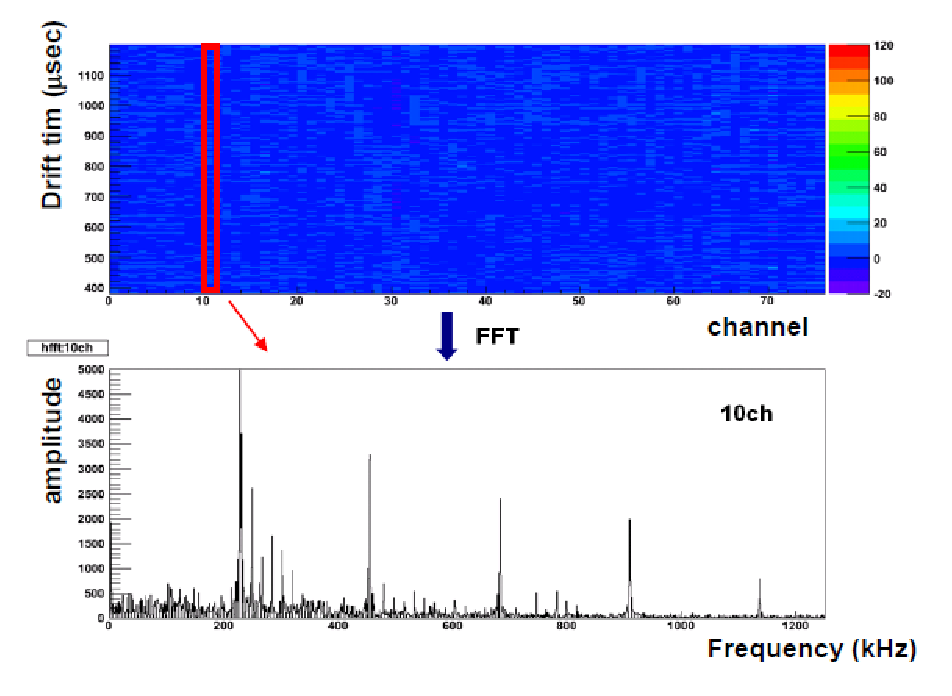
\includegraphics[width=11cm,clip]{./fig/example10ch.eps}
  \caption{example distribution of frequency:10ch}
  \label{example10ch}
\end{figure}
\begin{figure}[!htb]
  \centering
  \centering
  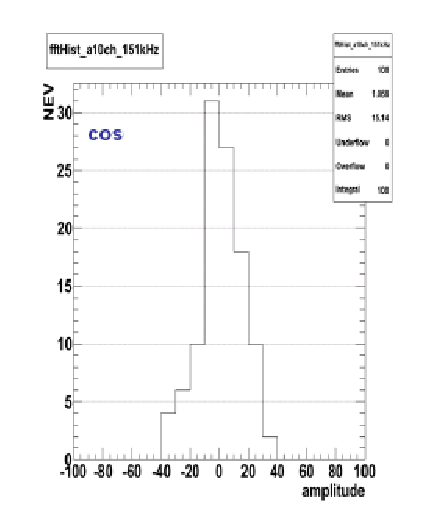
\includegraphics[width=11cm,clip]{./fig/cos.eps}
  \caption{An example of distribution of amplitude}
  \label{ampDist}
\end{figure}

\subsubsection{Making FFT noise}
 The procedure of making FFT noise is below:\\
\\
1. Get amplitude from the histograms of amplitude at random.\\
2. Perform Inverse FFT\\
\\
After performing inverse FFT, there is random noise (Fig\ref{randomNoise})which have the same distribution of frequency as real data. Real DATA have coherent noise but random noise don't have coherent components, therefore adding coherent components is necessary to reproduce realistic noise.\\
\\
3. Select random noise 0 and 32 and 64ch\\
4. Insert random noise 0 ch to 1-31ch, 32ch to 33-63ch, 64ch to 65-75ch\\
5. Scaling each channel \\
\\
Real DATA look having coherent noise board by board(We used 3 readout board in T32 experiment). We chosen 3 random noise(0ch,31ch,63ch) in this reason. After that, each channel needs to be corrected as each noise scale. Fig\ref{coherentNoise} shows coherent noise after scaling as Fig\ref{scaling}. Vertical axis of Fig\ref{scaling} is RMS of FADC, it stands for noise level.\\
\begin{figure}[!htb]
  \centering
  \centering
  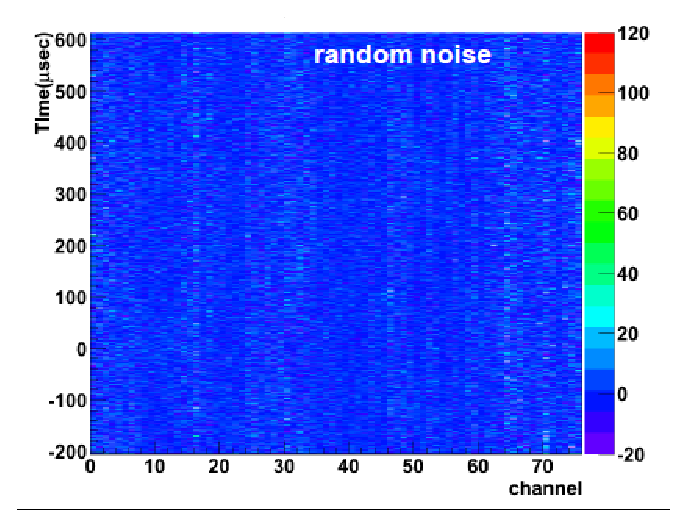
\includegraphics[width=11cm,clip]{./fig/randomnoise.eps}
  \caption{Random noise}
  \label{randomNoise}
\end{figure}
\begin{figure}[!htb]
  \centering
  \centering
  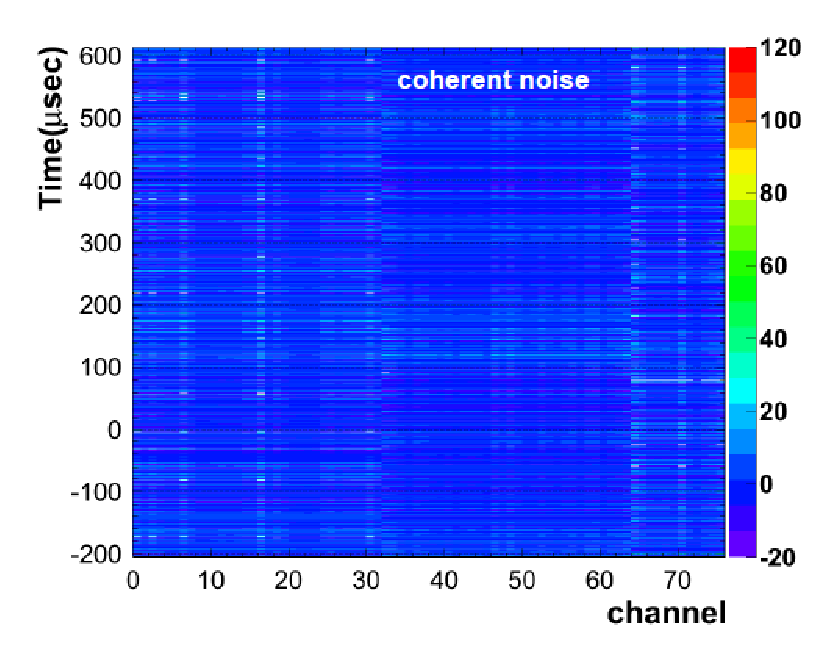
\includegraphics[width=11cm,clip]{./fig/coherentNoise.eps}
  \caption{Coherent noise}
  \label{coherentNoise}
\end{figure}
\begin{figure}[!htb]
  \centering
  \centering
  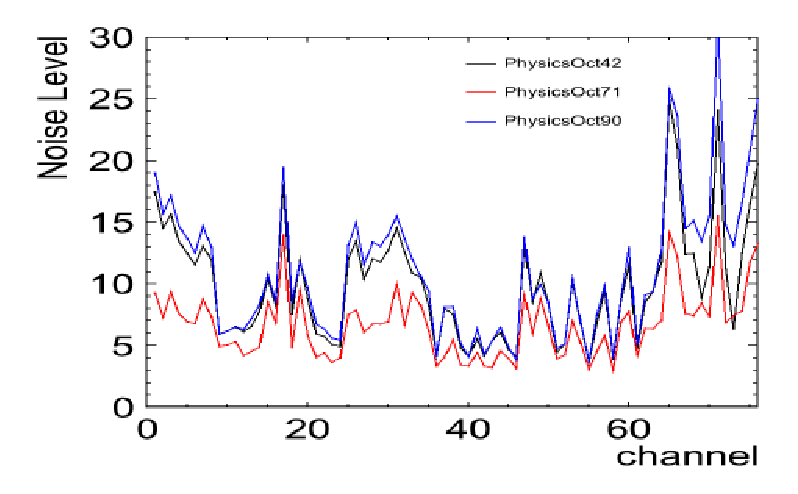
\includegraphics[width=11cm,clip]{./fig/scaling.eps}
  \caption{Noise level}
  \label{scaling}
\end{figure}
\\
6.Mixing Random noise and Coherent noise.\\
\\
Finally, We mixed Random noise and coherent noise as \\
\begin{equation}
  Realistic\,Noise = \frac{Random\,Noise + Coherent\,Noise}{2}
\end{equation}
